\documentclass[10pt]{beamer}
\usepackage{graphicx}
\usepackage{tikz}
\usepackage{lmodern}
\usepackage{mathtools}
\usepackage{amsmath,bm}
\usepackage{minted}
\usepackage[backend=bibtex]{biblatex}
\usepackage{hyperref}
\usepackage{multirow}

\usetheme{CambridgeUS}
\usecolortheme{seahorse}
\setbeamercovered{dynamic}
\usefonttheme{professionalfonts}
\setbeamertemplate{itemize items}[default]
\setbeamerfont{caption}{size=\footnotesize}
\addbibresource{bibliography.bib}
\setcounter{tocdepth}{2}

\newcommand*{\Scale}[2][4]{\scalebox{#1}{$#2$}}%
\newcommand*{\Resize}[2]{\resizebox{#1}{!}{$#2$}}%
%% Frame Title %%%%%%%%%%%%%%%%%%%%%%%%%%%%%%%%%%%
%\AtBeginSection[]
%{
%  \begin{frame}
%    \frametitle{Table of Contents}
%    \tableofcontents[currentsection]
%  \end{frame}
%}
%%%%%%%%%%%%%%%%%%%%%%%%%%%%%%%%%%%%%%%%%%%%%%%%%%

\begin{document}

\title[Compact finite differences on GPUs]
{A novel approach to evaluating 
compact finite differences 
and similar tridiagonal schemes on GPU-accelerated clusters}


\author[Ashwin Srinath]{
        Ashwin Srinath\\
        Department of Mechanical Engineering\\
        \today \newline \\
        \textbf{Committee members:} \\
        Dr. Gang Li \\
        Dr. Richard S. Miller \\
    Dr. Lonny Thompson}
\date{}
\titlepage

\begin{frame}{Overview}
    \tableofcontents
\end{frame}


\section{Motivation}

\begin{frame}
\frametitle{Introduction}
DNS: An approach for numerically solving
the Navier-Stokes equations
\begin{itemize}
\item Extremely fine computational grids
\item High-order accurate numerical schemes
\item e.g., \emph{compact} finite
    difference schemes for approximating derivatives
\item High computational cost
    \begin{itemize}
    \item Feasible only for simple flows
    \item Parallelism almost always required
    \end{itemize}
\end{itemize}
\end{frame}

\begin{frame}
\frametitle{Compact finite difference schemes}
A class of high-order accurate finite difference schemes
for evaluating spatial derivatives

\centering
\includegraphics[width=200px]{img/discretize-function.eps}

\begin{itemize}
\item {General form of compact schemes:
\begin{align*}
\begin{split}
f_i^{\prime} + \alpha(f^{\prime}_{i-1} + f^{\prime}_{i+1}) + \
\beta(f^{\prime}_{i-2} + f^{\prime}_{i+2}) + \hdots  = \
a\frac{f_{i+1} - f_{i-1}}{dx} + \\
b\frac{f_{i+2} - f_{i-2}}{dx} + \
c\frac{f_{i+3} - f_{i-3}}{dx} + \
    \hdots
\end{split}
\end{align*}}
\item $\alpha$, $\beta$, $a$, $b$, $\hdots$ must
    satisfy certain constraints
\item Derivative defined \emph{implicitly}
\end{itemize}
\end{frame}

\begin{frame}
\footnotesize
Solution strategy
\begin{itemize}
\item {Consider the specific scheme:
\begin{align*}
f_i^{\prime} + \frac{1}{4}(f^{\prime}_{i-1} + f^{\prime}_{i+1}) = \
\frac{3}{4}\frac{f_{i+1} - f_{i-1}}{dx}
\end{align*}}

\item {We write the expression for all points:
\begin{align*}
f_2^{\prime} + \frac{1}{4}(f^{\prime}_{1} + f^{\prime}_{3}) =
    \frac{3}{4}\frac{f_{3} - f_{1}}{dx} \\
%
f_3^{\prime} + \frac{1}{4}(f^{\prime}_{2} + f^{\prime}_{4}) =
    \frac{3}{4}\frac{f_{4} - f_{2}}{dx} \\
%
f_4^{\prime} + \frac{1}{4}(f^{\prime}_{3} + f^{\prime}_{5})
    = \frac{3}{4}\frac{f_{5} - f_{3}}{dx} \\
%
\hdots
%
f_{n-1}^{\prime} + \frac{1}{4}(f^{\prime}_{n-2} + f^{\prime}_{n})
    = \frac{3}{4}\frac{f_{n} - f_{n-2}}{dx}
\end{align*}}

\item {Special ``one-sided'' equations are needed near the boundaries:

\begin{align*}
f^{\prime}_1 + 2f^{\prime}_2 &= \frac{-5f_1 + 4f_2 + f_3}{dx} \\
%
f^{\prime}_{n} + 2f^{\prime}_{n-1}
&=
\frac{5f_{n} - 4f_{n-2} -  f_{n-1}}{dx}
\end{align*}}

\end{itemize}
\end{frame}

\begin{frame}[t]
\footnotesize
The full set of equations is expressed succinctly as:
\begin{equation*}
 \begin{bmatrix}
     1&2\\
     1/4&1&1/4\\
     &1/4&1&1/4\\
     &&1/4&1&1/4\\
     &&&1/4&1&1/4\\
     &&&&&\ddots\\
     &&&&&&\ddots\\
     &&&&&&&\ddots\\
     &&&&&&&2&1
  \end{bmatrix}
  \boxed{
  \begin{bmatrix}
      f^{\prime}_1 \\
      f^{\prime}_2 \\
      f^{\prime}_3 \\
      \vdots \\
      \vdots \\
      \vdots \\
      \vdots \\
      f^{\prime}_{n-1} \\
      f^{\prime}_n
   \end{bmatrix}
   }
 =
 \begin{bmatrix}
     \frac{-5f_1 + 4f_2 + f_3}{2dx}\\
     \frac{3(f_{3} - f_{1})}{4dx}\\
     \frac{3(f_{4} - f_{2})}{4dx}\\
     \vdots\\
     \vdots\\
     \vdots\\
     \vdots\\
     \frac{3(f_{n} - f_{n-2})}{4dx}\\
     \frac{5f_{n} - 4f_{n-1} - f_{n-2}}{2dx}
  \end{bmatrix}
\end{equation*}

Solution yields the derivatives at all points
$i=1,2, \hdots n$ simultaneously.
\begin{itemize}
\item In general, compact schemes yield banded systems
\item Tridiagonal schemes generally sufficient
\end{itemize}
\end{frame}

\begin{frame}
\frametitle{Objectives}
\begin{itemize}
    \item Exploratory work for exploiting GPUs
        in current research code
        \begin{itemize}
            \item important step for our group: Palmetto cluster
        currently has 598 GPUs (and counting)
        \end{itemize}
    \item An efficient GPU tridiagonal solver
    \item Parallelize the compact finite difference evaluation---current
        research code uses a sequential approach
\end{itemize}
\end{frame}

\begin{frame}
\frametitle{Thesis contributions}
\begin{itemize}
    \item A novel solution strategy for
        the tridiagonal systems arising in
        compact finite differences
        and other numerical schemes
    \item A strategy for evaluating compact
        finite differences on GPU-accelerated clusters
\end{itemize}
\end{frame}



\subsection{Graphics processing units}

\begin{frame}[t]
\frametitle{Introduction}
\pause
\begin{columns}[T]
\begin{column}{0.4\textwidth}
\begin{itemize}
    \item <2-> Highly multi-threaded processor
        \begin{itemize}
            \item NVIDIA Tesla K20 accelerator: 2496 cores
        \end{itemize}
    \item <3-> Spectacular performance for
        \emph{compute-intensive, data-parallel} operations
    \item <4-> Not suited for general-purpose computation
    \item <5-> Requires careful redesign of algorithms,
        substantial code changes, and tuning efforts
\end{itemize}
\end{column}
\begin{column}{0.6\textwidth}
\visible<2-> {
    \vspace{2cm}
    \includegraphics[width=180px]
    {img/device-comparison.png}
}
\end{column}
\end{columns}
\end{frame}

\begin{frame}
\frametitle{Programming GPUs}
\pause
Scientific applications use GPUs at various levels:
\begin{itemize}
    \item Low-level
        \begin{itemize}
            \item CUDA
            \item OpenCL
        \end{itemize}
    \item High-level
        \begin{itemize}[<+->]
            \item OpenACC compiler directives
            \item Drop-in support for scientific libraries such as Intel MKL, BLAS
        \end{itemize}
    \item Transparent
        \begin{itemize}[<+->]
            \item MATLAB: over 200 functions
            \item Software packages: Abaqus, ANSYS (Mechanical/Fluent)
        \end{itemize}
\end{itemize}
\end{frame}

\begin{frame}
\frametitle{CUDA programming model}
\pause
\begin{columns}
\begin{column}{0.5\textwidth}
\textbf{Kernels}
\begin{itemize}[<+->]
    \item Special pieces of code that execute on the GPU
    \item In Fortran: subroutines; in C: functions
    \item Executed concurrently by several GPU threads
\end{itemize}
\textbf{Threads}
\begin{itemize}[<+->]
    \item Threads organized into a grid of blocks
    \item Kernels launched with specified grid size
        (number of blocks) and block size (threads per block)
    \item Grid and blocks can be 2-D or 3-D for convenience
\end{itemize}
\end{column}
\begin{column}{0.5\textwidth}
    \only<5-6>{\includegraphics[width=150px]{img/program-structure.png}}
    \only<7>{\includegraphics[width=150px]{img/grid-of-thread-blocks.png}}
\end{column}
\end{columns}
\end{frame}

\begin{frame}
\frametitle{GPU architecture and memory model}
\pause
\begin{columns}
\begin{column}{0.5\textwidth}
\begin{itemize}[<+->]
    \item GPU viewed as a collection of \emph{streaming microprocessors} (SMs)
    \item When kernel is launched, each block gets assigned to an SM
    \item Threads within a block execute concurrently
    \item SM may execute several blocks concurrently
\end{itemize}
\end{column}
\begin{column}{0.5\textwidth}
    \visible<3->{\includegraphics[width=150px]{img/gpu-scaling.png}}
\end{column}
\end{columns}
\end{frame}

\begin{frame}
\frametitle{GPU architecture and memory model}
\pause
\begin{columns}
\begin{column}{0.5\textwidth}
\begin{itemize}
    \item Global memory{
        \begin{itemize}
            \item large but slow (~5 GB for Tesla K20)
            \item all threads can access
            \item persists between kernel launches
        \end{itemize}}
    \item Shared memory{
        \begin{itemize}
            \item small but fast (~48 KiB per SM)
            \item local to threads within a block
            \item explicitly managed cache
        \end{itemize}}
    \item Registers{
        \begin{itemize}
            \item limited (65536 per SM)
            \item local to individual threads
            \item fastest
        \end{itemize}}
\end{itemize}
\end{column}
\begin{column}{0.5\textwidth}
    \visible<2->{\includegraphics[width=150px]{img/memory-hierarchy.png}}
\end{column}
\end{columns}
\end{frame}


\section{Developing a tridiagonal solver}

\begin{frame}
\frametitle{Requirements of tridiagonal solver}

Each line of grid points yields a tridiagonal system:
\small
\begin{equation*}
 \begin{bmatrix}
     1&2\\
     1/4&1&1/4\\
     &1/4&1&1/4\\
     &&1/4&1&1/4\\
     &&&1/4&1&1/4\\
     &&&&&\ddots\\
     &&&&&&\ddots\\
     &&&&&&&\ddots\\
     &&&&&&&2&1
  \end{bmatrix}
  \begin{bmatrix}
      f^{\prime}_1 \\
      f^{\prime}_2 \\
      f^{\prime}_3 \\
      \vdots \\
      \vdots \\
      \vdots \\
      \vdots \\
      f^{\prime}_{n-1} \\
      f^{\prime}_n
   \end{bmatrix}
 =
 \begin{bmatrix}
     \frac{-5f_1 + 4f_2 + f_3}{2dx}\\
     \frac{3(f_{3} - f_{1})}{4dx}\\
     \frac{3(f_{4} - f_{2})}{4dx}\\
     \vdots\\
     \vdots\\
     \vdots\\
     \vdots\\
     \frac{3(f_{n} - f_{n-2})}{4dx}\\
     \frac{5f_{n} - 4f_{n-1} - f_{n-2}}{2dx}
  \end{bmatrix}
\end{equation*}
\end{frame}

\begin{frame}
\frametitle{Requirements of tridiagonal solver}
\begin{columns}
\begin{column}{0.5\textwidth}
\begin{itemize}
\item For a 1-D grid, solution gives the derivative
    at all points simultaneously
\item For 2-D and 3-D grids, we solve a tridiagonal system
    for each grid line
\item The coefficient matrix is the same for each system
\item Only right hand sides are different
\end{itemize}
\end{column}
\begin{column}{0.5\textwidth}
    \hspace{1cm}
    \includegraphics[width=100px]{img/grid-lines.eps}
\end{column}
\end{columns}
\end{frame}

\begin{frame}
\frametitle{Thomas algorithm}
\begin{itemize}
\item Derived from Gaussian elimination
\item Requires $2n$ steps and $4n$ storage
\item The most efficient serial implementation
\item What about for GPUs?
    \begin{itemize}
        \item inherently sequential
        \item can use multiple threads to solve
            individual tridiagonal systems
    \end{itemize}
\end{itemize}
\end{frame}

\begin{frame}
\frametitle{Issues with GPU implementation}
\begin{columns}
\begin{column}{0.5\textwidth}
\begin{itemize}
    \item Uncoalesced global memory accesses
    \item What about shared memory?
        \begin{itemize}
            \item 4N storage \emph{per block}
            \item SM shared memory filled up quickly
            \item very few threads per SM
            \item under-utilizes the GPU parallelism
        \end{itemize}
    \item $2n$ steps - can do better on GPU
\end{itemize}
\end{column}
\begin{column}{0.5\textwidth}
    \includegraphics[width=150px]{img/pThomas.eps}
\end{column}
\end{columns}
\end{frame}

\begin{frame}
\frametitle{Tridiagonal solvers for the GPU}
\begin{itemize}
\item Zhang et al. (2010) describe the implementation
    of three algorithms for tridiagonal systems on GPUs
    \begin{itemize}
        \item Cyclic reduction
        \item Parallel cyclic reduction
        \item Recursive doubling
    \end{itemize}
\item Exhibit \emph{fine-grained} parallelism
\item Subsequent efforts based on CR and PCR primarily
\end{itemize}
\end{frame}

\begin{frame}
\frametitle{Cyclic reduction}
\begin{columns}
\begin{column}{0.5\textwidth}
\begin{itemize}
\item Buzbee and Goleb (1970)
\item \textbf{Forward reduction} ($log(n)-1$ steps):
    \begin{itemize}
    \item Eliminate odd-indexed equations at each step
    \item Two-by-two system is left
    \end{itemize}
\item \textbf{Backward substitution} ($log(n)-1$ steps):
    \begin{itemize}
    \item Solve for odd-indexed equations using even-indexed values
    \end{itemize}
\item Best case ($n$ parallel threads): requires $2log(n)-1$ steps
\end{itemize}
\end{column}
\begin{column}{0.5\textwidth}
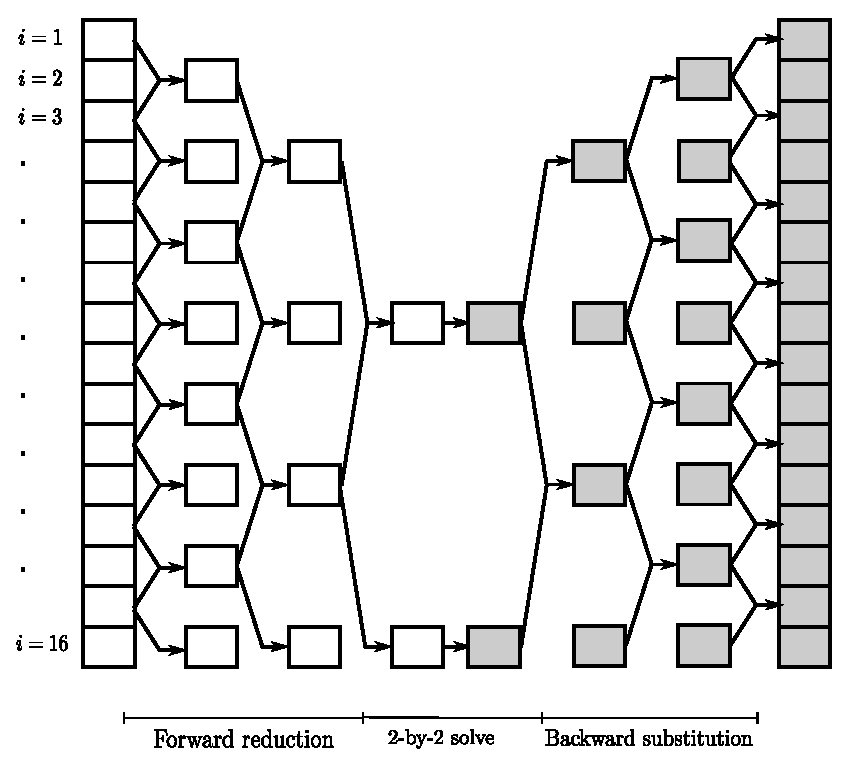
\includegraphics[width=150px]{img/cyclic-reduction.eps}
\end{column}
\end{columns}
\end{frame}

\begin{frame}
\frametitle{GPU implementation}
\begin{columns}
\begin{column}{0.5\textwidth}
\begin{itemize}
\item Each tridiagonal system mapped to a thread block;
    individual threads mapped to equations
\item Several systems can be solved at concurrently
\item Forward reduction: diagonal arrays $a$, $b$, $c$ and RHS $d$
    updated \emph{in-place}
\item Backward substitution: solution $x$ computed
    from $a^\prime$, $b^\prime$, $c^\prime$ and $d^\prime$
\item Synchronization required at each step
\end{itemize}
\end{column}
\begin{column}{0.5\textwidth}
\only<1>{
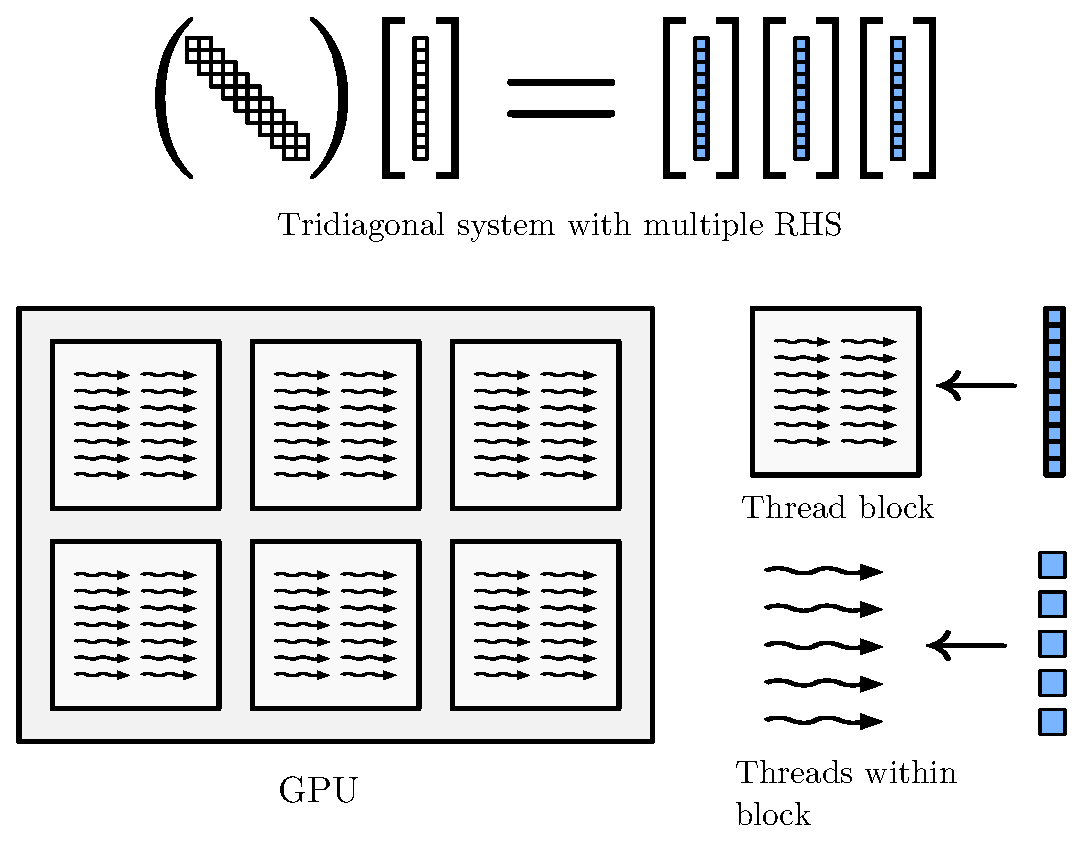
\includegraphics[width=150px]{img/gpu-mapping.eps}
}
\only<2>{
\centering
Forward reduction
\scalebox{0.8}{
\vbox{
\begin{align*} 
    k_1 &= \frac{a_i}{b_{i-1}}, k_2 = \frac{c_i}{b_{i+1}} \\
    a^{\prime}_i &= -a_{i-1}k_1 \\
    b^{\prime}_i &= b_i - c_{i-1}k_1 - a_{i+1}k_2 \\
    c^{\prime}_i &= -c_{i+1}k_2 \\
    d^{\prime}_i &= d_i - d_{i-1}k_1  - d_{i+1}k_2 \\
\end{align*}}}

\centering
Backward substitution
\scalebox{0.8}{
\vbox{
\begin{align*}
x_i &= \frac{d^{\prime}_i - a^{\prime}_ix_{i-1} - \
    c^{\prime}_ix_{i+1}}{b^{\prime}_i}
\end{align*}}}}

\end{column}
\end{columns}
\end{frame}

\begin{frame}
\frametitle{Issues}
\begin{columns}
\begin{column}{0.5\textwidth}
\begin{itemize}
    \item Thread activity
    \item Uncoalesced global memory access
    \item Bank conflicts
    \item Limited shared memory
\end{itemize}
\end{column}
\begin{column}{0.5\textwidth}
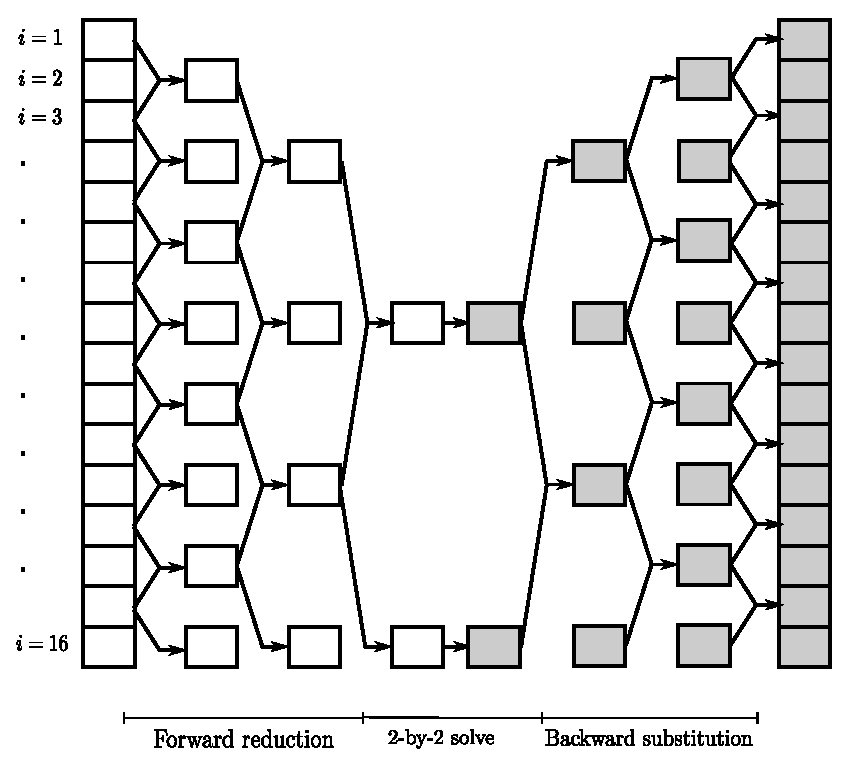
\includegraphics[width=150px]{img/cyclic-reduction.eps}
\end{column}
\end{columns}
\end{frame}

\begin{frame}
\frametitle{Efforts for improving performance}
\begin{itemize}
    \item Zhang et al.: hybrid CR+PCR solver
    \item G{\"o}ddeke et al.: separate even and odd indexed
        coefficients
    \item Davidson et al.: register packing
    \item Esfahanian et al.: global memory with data rearrangement
\end{itemize}
\end{frame}

\begin{frame}
\frametitle{A novel approach}
\begin{itemize}
\item Solving systems with same RHS
\item Computing $a^\prime$, $b^\prime$ and $c^\prime$
    for each system and at every time step redundant
\item Storing coefficients (similar to LU) - expensive
\item The coefficient matrix has relatively simple structure
\item Can be exploited to improve cyclic reduction performance
\end{itemize}
\end{frame}

\begin{frame}
\begin{columns}
\begin{column}{0.5\textwidth}
\begin{itemize}
    \item Diagonals are nearly constant (\emph{near-Toeplitz})
    \item Symmetry may be broken by boundary conditions
    \item Near-Toeplitz matrices occur in other numerical schemes
    \begin{itemize}
        \item Alternating direct implicit methods
        \item Line relaxation methods
        \item Poisson solvers
        \item One-dimensional ODEs and PDEs
    \end{itemize}
\end{itemize}
\end{column}
\begin{column}{0.5\textwidth}
\centering
\scalebox{0.6}{%
\vbox{
\begin{equation*}
\begin{bmatrix}
     1&2\\
     1/4&1&1/4\\
     &1/4&1&1/4\\
     &&1/4&1&1/4\\
     &&&1/4&1&1/4\\
     &&&&&\ddots\\
     &&&&&&\ddots\\
     &&&&&&&\ddots\\
     &&&&&&&2&1
  \end{bmatrix}
\end{equation*}}}
\end{column}
\end{columns}
\end{frame}

\begin{frame}
\frametitle{General approach}
\begin{columns}
\begin{column}{0.5\textwidth}
\begin{itemize}
\item {First reduction step, substitute:
    \scalebox{0.8}{
    \vbox{
    \begin{align*}
        a_2 &= a_3 = a_4 = \hdots &\equiv a_0 \\
        b_2 &= b_3 = b_4 = \hdots &\equiv b_0 \\
        c_2 &= c_3 = c_4 = \hdots &\equiv c_0
    \end{align*}}}}
\item $a^\prime$, $b^\prime$, $c^\prime$
    represent coefficients of the ``reduced'' tridiagonal system
\item \textbf{The reduced system is also near-Toeplitz}
\item Each forward reduction step produces a near-Toeplitz
    tridiagonal system
\item Coefficients can be stored compactly
\end{itemize}
\end{column}
\begin{column}{0.5\textwidth}
\centering
Forward reduction
\scalebox{0.8}{
\vbox{
\begin{align*} 
    k_1 &= \frac{a_i}{b_{i-1}}, k_2 = \frac{c_i}{b_{i+1}} \\
    a^{\prime}_i &= -a_{i-1}k_1 \\
    b^{\prime}_i &= b_i - c_{i-1}k_1 - a_{i+1}k_2 \\
    c^{\prime}_i &= -c_{i+1}k_2 \\
    d^{\prime}_i &= d_i - d_{i-1}k_1  - d_{i+1}k_2 \\
\end{align*}}}
\end{column}
\end{columns}
\end{frame}

\begin{frame}
Cyclic reduction reduced to:

\vspace{1cm}

\textbf{Forward reduction}
\begin{align*}
d^{\prime}_i = d_i - d_{i-1}k_1^{m}  - d_{i+1}k_2^{m}
\end{align*}

\textbf{Backward substitution}
\begin{align*}
x_i = \frac{d^{\prime}_i - a^mx_{i-1} - \
    c^{m}x_{i+1}}{b^m}
\end{align*}

where $a^m$, $b^m$ and $c^m$ are the precomputed
coefficients for $i>1$ at the step $m$.
\end{frame}



\section{Application to compact finite differences}

\begin{frame}
\frametitle{Application to compact finite difference schemes}
\begin{itemize}
\item Compact finite difference evaluation involves two steps:
\begin{enumerate}
\item Evaluation of the right hand sides
\begin{itemize}
    \item easily performed on the GPU
\end{itemize}
\item Solving the tridiagonal systems for all the grid lines
\end{enumerate}
\item Current efforts:
\begin{itemize}
    \item Tutkun et al. (2012)
    \item Esfahanian et al. (2014)
\end{itemize}
\item Typical DNS problems too large to fit on a single GPU
\item Need a strategy for multiple GPUs
\end{itemize}
\end{frame}

\begin{frame}
\frametitle{Parallelization strategy: multiple GPUs on a single node}
\begin{columns}
\begin{column}{0.5\textwidth}
\begin{itemize}
\item Method used by Sakharnykh et al.
\item Decompose domain into \emph{subdomains};
    each GPU assigned a subdomain
\item Single subdomain used along derivative direction
\item No coordination between GPUs required
\item For other coordinate directions,
    transpose the data (physically or logically)
\end{itemize}
\end{column}
\begin{column}{0.5\textwidth}
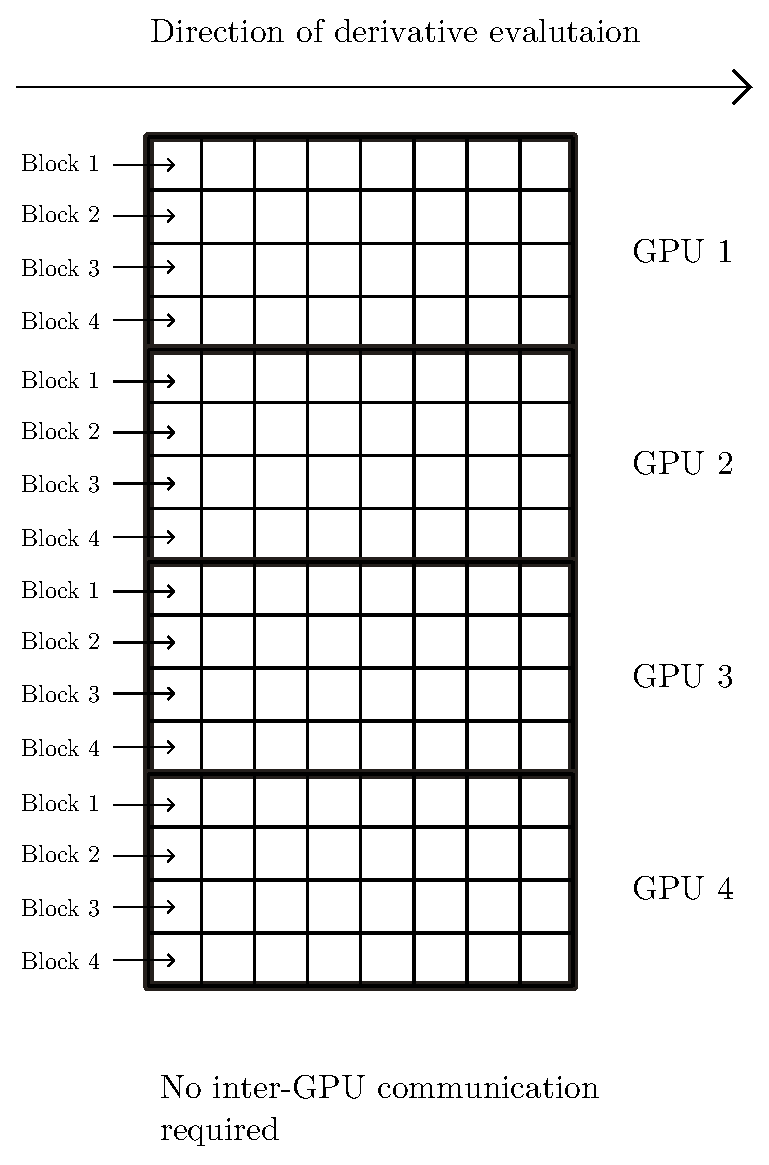
\includegraphics[width=100px]{img/compact-shared-gpu.eps}
\end{column}
\end{columns}
\end{frame}

\begin{frame}
\frametitle{Parallelization strategy: multiple GPUs on distinct nodes}
\begin{columns}
\begin{column}{0.5\textwidth}
\begin{itemize}
\item Single subdomain used along derivative direction
\item No coordination between GPUs required
\item \textbf{Physical} global transpose required
\item Subdomains can become impractically slender
\item Scalable approach needs a distributed tridiagonal solver
\end{itemize}
\end{column}
\begin{column}{0.5\textwidth}
    \only<1>{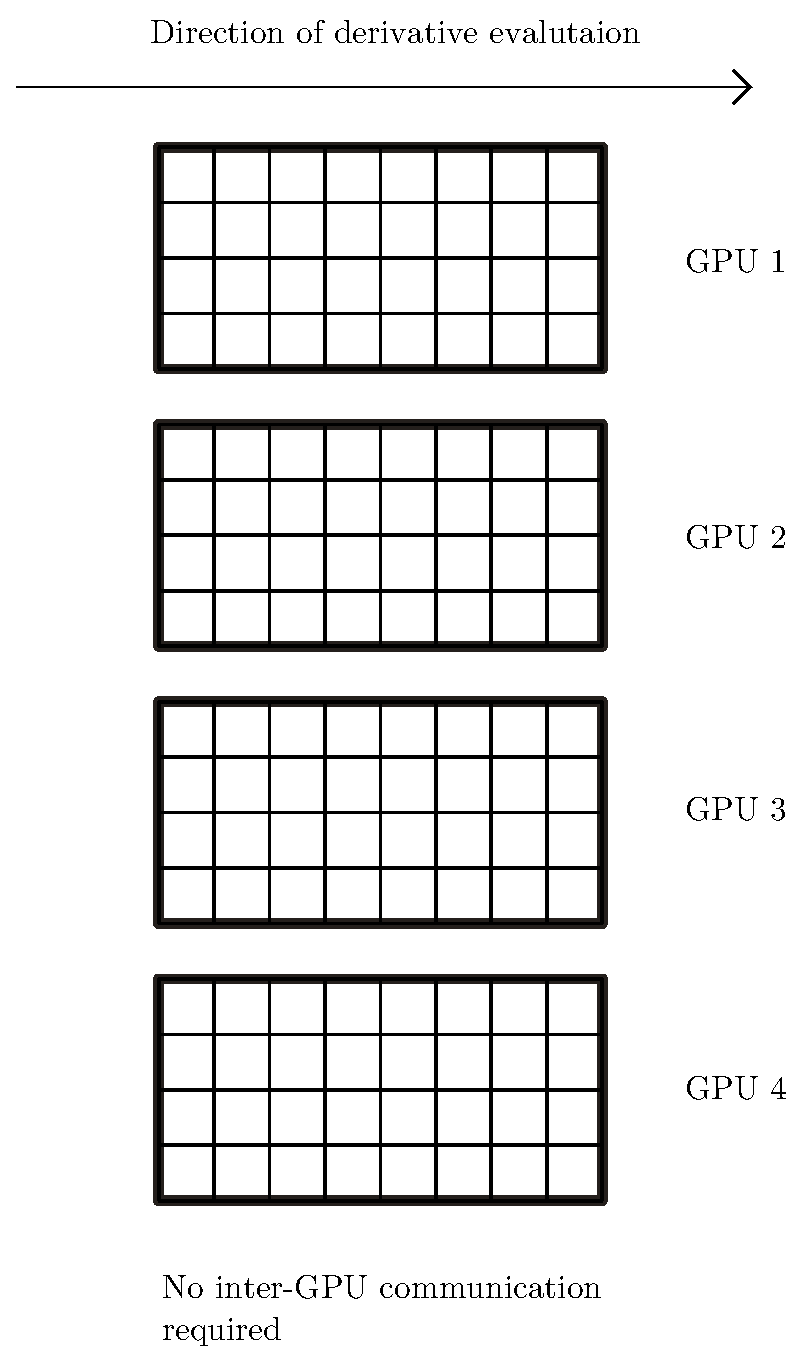
\includegraphics[width=100px]{img/compact-distributed-restricted.eps}}
    \only<2>{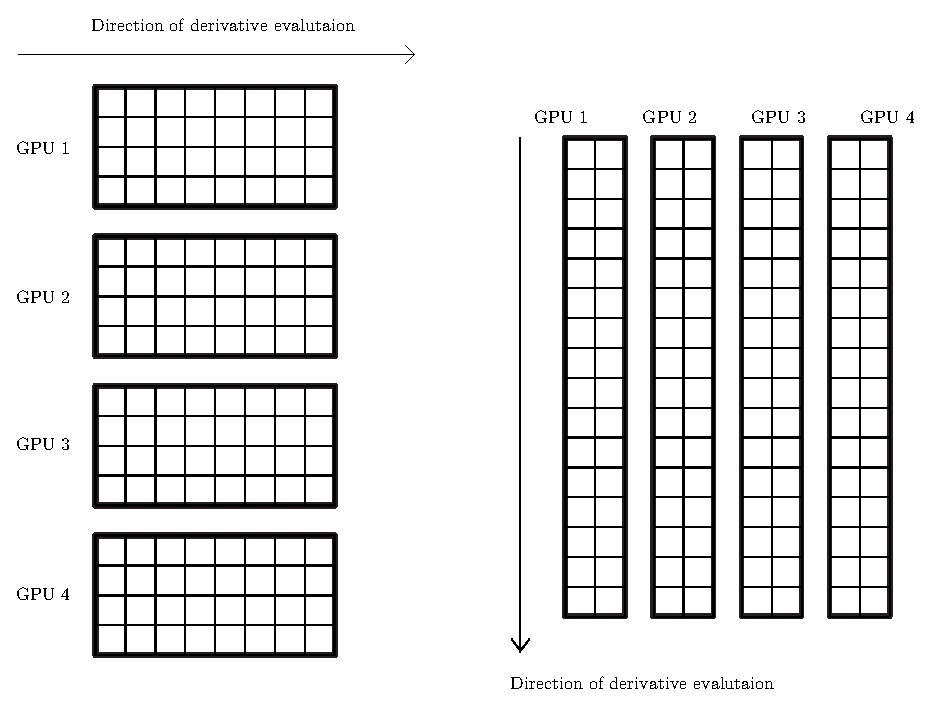
\includegraphics[width=150px]{img/compact-restricted-transpose.eps}}
    \only<3>{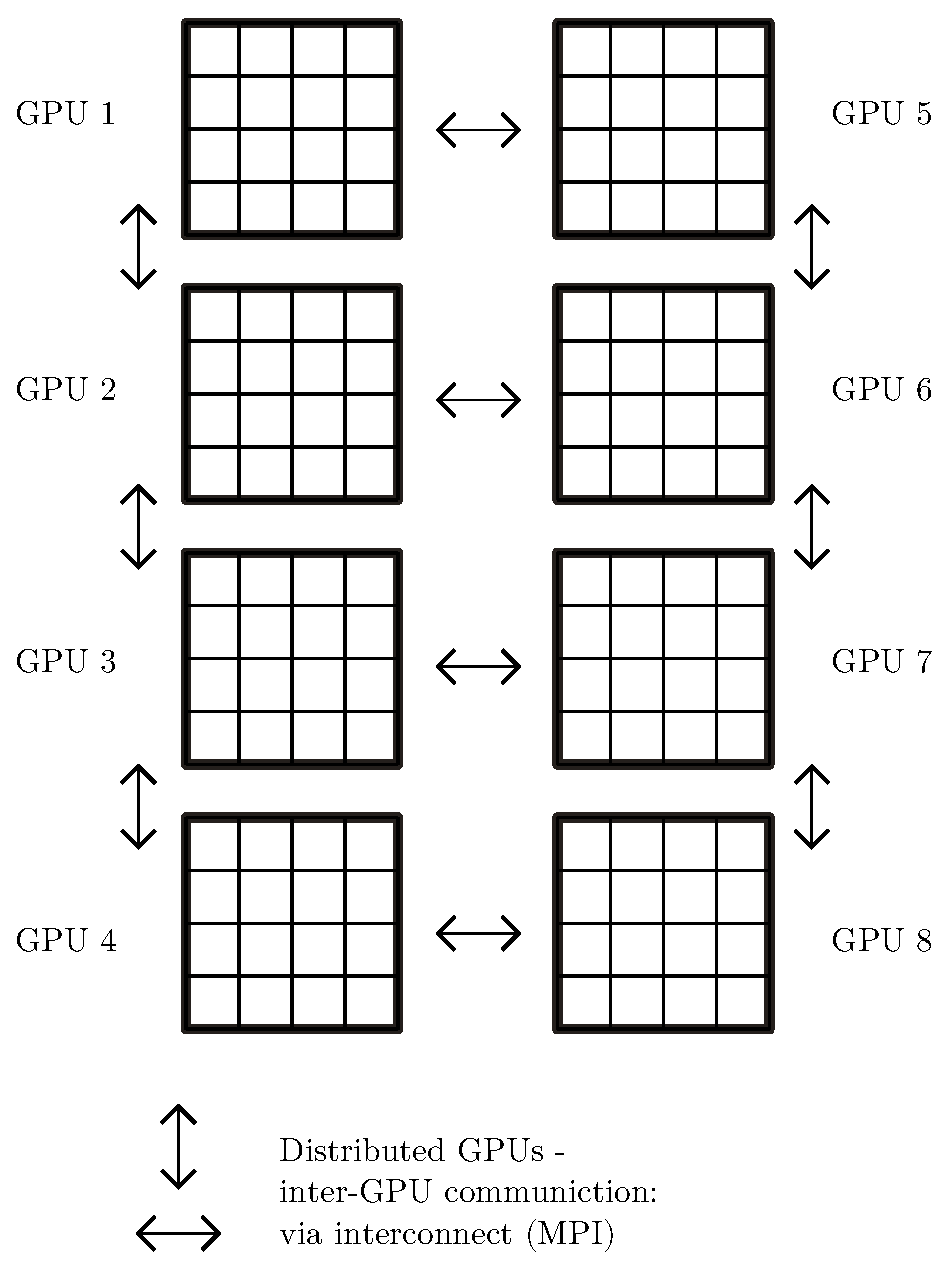
\includegraphics[width=120px]{img/compact-distributed-all.eps}}
\end{column}
\end{columns}
\end{frame}

\begin{frame}
\frametitle{Distributed tridiagonal solver}

Solving a tridiagonal system of size
$mP$, split among $P$ processes (Mattor et al., 1995):

\footnotesize
\begin{columns}
\begin{column}{0.5\textwidth}
\begin{enumerate}
\item Each process solves the local systems:
    \begin{align*}
        A^px_r^{p} &= r_p \\
        A^pu^p &= \{-a_1^p, 0, 0, 0, \hdots\} \\
        A^pl^p &= \{0, 0, 0 \hdots, -c_m^p\}
    \end{align*}
\item Construct and assemble a ``reduced'' system
    of the form:
    \scalebox{0.6}{
        \vbox{
    \begin{align*}
     \begin{bmatrix}
l^1_m & -1 \\
-1    & u^2_1 & l^2_1 \\
  & u^2_m & l^2_m & -1 \\
  &       & -1    & u^3_1 & l^3_1 \\
  &       &       & u^3_m & l^3_m  & -1 \\
  &       &       &       & \ddots & \ddots & \ddots \\
  &       &       &       &        & -1     & u^P_1
\end{bmatrix}
\begin{bmatrix}
\beta^1 \\
\alpha^2 \\
\beta^2 \\
\alpha^3 \\
\beta^3 \\
\vdots \\
\alpha^P
\end{bmatrix}
=
\begin{bmatrix}
x_{r,m}^1 \\
x_{r,1}^2 \\
x_{r,m}^2 \\
x_{r,1}^3 \\
x_{r,m}^3 \\
\vdots \\
x_{r,1}^P \\
\end{bmatrix}  
        \end{align*}}}
\item Local part of solution given by:
\begin{align*}
x^p = x_r^p + \
    \alpha^p u^p + \beta^p l^p
\end{align*}
\end{enumerate}
\end{column}
\begin{column}{0.5\textwidth}
\centering
\includegraphics[width=120px]{img/dividing-tridiagonal.eps}
\end{column}
\end{columns}
\end{frame}

\begin{frame}
\frametitle{Compact finite difference on multi-GPU system}
\footnotesize
\begin{columns}
\begin{column}{0.5\textwidth}
\begin{enumerate}
\item Computing RHS for all local grid points - \textbf{requires communication}
\begin{itemize}
    \footnotesize
    \item halo swaps with neighbouring GPUs
    \item pointwise stencil
\end{itemize}
\item Solving local tridiagonal systems - no communication
\item Assembling and solving reduced tridiagonal systems - \textbf{requires communication}
\begin{itemize}
    \footnotesize
    \item global communication along line of GPUs
    \item produces interleaved tridiagonal sysems - pThomas algorithm
\end{itemize}
\item Summing solutions from steps 2 and 3 - no communication
\begin{itemize}
    \footnotesize
    \item pointwise sum
\end{itemize}
\item For other coordinate directions: \emph{local} permutation of data
\end{enumerate}
\end{column}
\begin{column}{0.5\textwidth}
\only<1>{\includegraphics[width=175px]{img/rhs-halos.eps}}
\only<2>{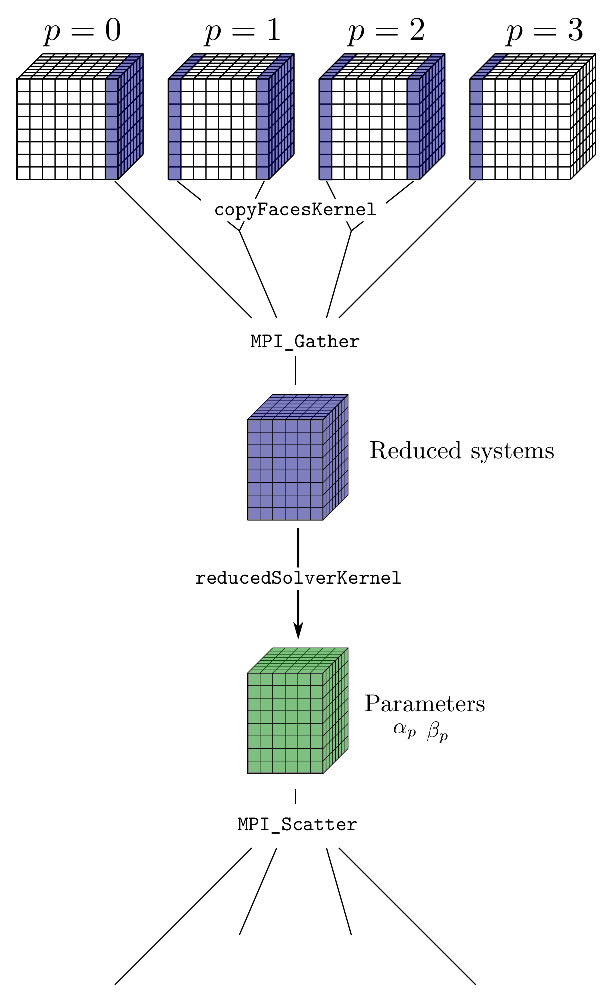
\includegraphics[width=175px]{img/constructing-reduced-system.eps}}
\end{column}
\end{columns}
\end{frame}



\chapter{Results}

\section{Performance of GPU tridiagonal solver}

In this section we present a performance overview
of our NEATO solver
against a multi-threaded Intel MKL solver and
the CUSPARSE GPU solver
(\texttt{dgtsv} and \texttt{dgtsvStridedBatch} respectively).
The MKL solver uses Gaussian elimination with partial pivoting,
and the CUSPARSE solver uses a combination of
Cyclic Reduction and Parallel Cyclic Reduction
as described by Zhang et al. \cite{Zhang2010FTS}.
These solvers represent the most straightforward way
to compute solutions for tridiagonal systems
and are highly optimized for performance on
underlying architectures.
Boundary conditions may prevent
the matrix from being symmetric and/or diagonally dominant,
precluding the use of more specialized tridiagonal solvers.

The CPU code is compiled with the Intel C compiler (version 15.0),
and run (with OpenMP support) on up to
16 independent cores of the the same shared-memory node
(one thread per core).
The CPU is an
Intel Xeon Processor E5-2670 v2 (2.50 GHz, 25 MB Smart Cache).
GPU code is compiled with the CUDA toolkit (version 6.5.14),
and run on the
NVIDIA Tesla K20 Accelerator.
When measuring GPU performance (both CUSPARSE and NEATO),
we do \emph{not} include the cost
of data transfer between the CPU and GPU.
This is because the tridiagonal solver is expected to be
part of a larger application.
This is in keeping with the timing strategies
in related literature.

The \texttt{-O2} level compiler optimizations are turned on for both
CPU and GPU code;
no further optimization options are enabled in either case.
Of course, we use double precision for all solvers.
The timings reported are
kernel \emph{execution} times, i.e.,
the time for all kernel(s) to execute completely
before returning the program control to the CPU.
All timings are averaged over 100 tridiagonal solves.

\subsection{NEATO: global memory v/s shared memory performance}

\begin{figure}[h]
\begin{center}
\includegraphics[width=300pt]{fig/global-vs-shared-2d.eps}
\caption{Comparison of global memory and shared
    memory implementations of NEATO (2D problems).}
\label{fig:global-vs-shared-2d}
\end{center}
\end{figure}

\begin{figure}[h]
\begin{center}
\includegraphics[width=300pt]{fig/global-vs-shared-3d.eps}
\caption{Comparison of global memory and shared memory
    implementations of NEATO (3D problems).}
\label{fig:global-vs-shared-3d}
\end{center}
\end{figure}

In Figs. \ref{fig:global-vs-shared-2d} and \ref{fig:global-vs-shared-3d},
we report the performance of the two solvers for the case
$N_{rhs} = n$ and $N_{rhs} = n^2$.
These cases correspond to tridiagonal systems
arising in 2-D and 3-D problems respectively.
We note that the shared memory implementation
offers better performance in nearly all cases.
However, the relative speedup from using
shared memory diminishes with increasing problem size.
For larger problem sizes,
the synchronization costs associated with inactive threads
leads to poor shared memory performance.

\subsection{Comparison of NEATO with Intel MKL and CUSPARSE solvers}

\begin{figure}
\begin{center}
\includegraphics[width=300pt]{fig/bench-2d.eps}
\caption{Relative solver performance for 2-D problems. Relative time defined as:}
Time taken by solver/Time taken by NEATO solver
\label{fig:bench-2d}
\end{center}
\end{figure}

\begin{figure}
\begin{center}
\includegraphics[width=300pt]{fig/bench-3d.eps}
\caption{Relative solver performance for 3-D problems. Relative time defined as:}
Time taken by solver/Time taken by NEATO solver
\label{fig:bench-3d}
\end{center}
\end{figure}

In Fig. \ref{fig:bench-2d} and \ref{fig:bench-3d},
we provide the relative performance of
Intel MKL and CUSPARSE solvers and compare against
the NEATO shared memory implementation.
The relative performance for
each problem size is obtained by
normalizing the solver timings
by the timing for the NEATO solver for that problem size.
Table \ref{table:bench} shows the timings of the various
solvers to solve different problem sizes.
Note that data is missing for the CUSPARSE solver
for the $512^3$ 3-D case,
as the GPU was unable to accomodate this problem size---this
is due to the large amount of scratch space required
by the CUSPARSE implementation.

\begin{sidewaystable}[]
\scriptsize
\centering
\caption{Performance of Intel MKL, CUSPARSE and NEATO solvers.}
\label{table:bench}
% Please add the following required packages to your document preamble:
% \usepackage{multirow}
\begin{tabular}{|l|l|l|l|l|l|l|}
\hline
\multirow{2}{*}              & \multirow{2}{*}{}        & \multicolumn{5}{c|}{Time to solve (ms)}                             \\ \cline{3-7}
\centering System size       & Number of systems        & MKL 1 core    & MKL 8  cores & CUSPARSE & NEATO (global) & NEATO (shared) \\ \hline
32                           & 32                       & 0.045         & 0.042         & 0.273    & 0.201          & 0.024          \\ \hline
64                           & 64                       & 0.048         & 0.048        & 0.271    & 0.247          & 0.025          \\ \hline
128                          & 128                      & 0.089         & 0.084        & 0.271    & 0.284          & 0.032          \\ \hline
256                          & 256                      & 0.263         & 0.107        & 0.305    & 0.326          & 0.066          \\ \hline
512                          & 512                      & 0.959         & 0.299        & 0.629    & 0.403          & 0.272          \\ \hline
1024                         & 1024                     & 3.775         & 1.023        & 1.939    & 1.375          & 1.252          \\ \hline
2048                         & 2048                     & 16.272        & 4.823        & 7.607    & 5.811          & 10.407         \\ \hline
32                           & 1024                     & 0.152         & 0.094        & 0.31     & 0.207          & 0.092          \\ \hline
64                           & 4096                     & 0.879         & 0.306        & 0.556    & 0.751          & 0.409          \\ \hline
128                          & 16384                    & 7.052         & 2.553        & 3.128    & 3.669          & 2.225          \\ \hline
256                          & 65536                    & 63.858        & 18.792       & 28.495   & 21.148         & 12.565         \\ \hline
512                          & 262144                   & 515.792       & 196.748      &          & 145.34         & 125.311        \\ \hline 
\end{tabular}

\end{sidewaystable}

\section{Performance of compact finite difference application}

The timings for the
compact finite difference application
were measured on the
Clemson University Palmetto Cluster,
using NVIDIA Tesla K20 and K40 GPUs.
The K40 GPUs were used for the largest problem sizes.
Each compute node on the cluster is equipped with up to 2 GPUs,
and nodes are connected by 56 Gbps Infiniband interconnect.
We use Open MPI 1.8.1 configured with OpenFabrics support.

The timings reported are \emph{wall clock} times
with global synchronization between processes performed 
before and after evaluation of the derivatives.
All timings are averaged over 100 evaluations of the function derivatives
in each coordinate direction.
We make it clear that our reported
problem sizes represent the \emph{actual size of problem data}.
Although it may be considered sufficient to
run tests on a single line of processes
for measuring the compact finite difference solver performance,
we set up and solve the problem for the entire computational domain.
In the context of a larger simulation,
global synchronization between the processes
is typically performed before and after the evaluation of derivatives,
and it is important to consider the related overhead.

\subsection{Performance profiling}

\begin{figure}[h!]
\begin{center}
\includegraphics[width=300pt]{fig/profiling-1024-64.eps}
\caption{Solving problem sized $1024^3$ on 64 GPUs}
\label{fig:compact-profiling-1024-64}
\end{center}
\end{figure}
%
\begin{figure}[h!]
\begin{center}
\includegraphics[width=300pt]{fig/profiling-2048-64.eps}
\caption{Solving problem sized $2048^3$ on 64 GPUs}
\label{fig:compact-profiling-2048-64}
\end{center}
\end{figure}
%
Figures \ref{fig:compact-profiling-1024-64} - \ref{fig:compact-profiling-2048-64}
show the time taken by the different steps of
the compact finite difference solver.
We note that for the larger problem size,
the evaluation of the primary systems (using the NEATO solver)
constitutes a larger majority of the total runtime,
which justifies our efforts in optimizing the tridiagonal solver.
For evaluation of the derivatives in the $y-$ and $z-$ directions,
we note that a significant portion of the runtime is dedicated
to performing permutations of the input and output data.
We attribute this to our na\"{\i}ve implementation of the
permutation kernels (no shared memory usage).

\subsection{Strong and weak scaling}
\begin{figure}
\begin{center}
\includegraphics[width=300pt]{fig/strong-scaling-256.eps}
\caption{Strong scaling for multi-GPU compact finite difference, problem size: $256^3$.}
\label{fig:strong-scaling-256}
\end{center}
\end{figure}
%
\begin{figure}
\begin{center}
\includegraphics[width=300pt]{fig/strong-scaling-512.eps}
\caption{Strong scaling for multi-GPU compact finite difference, problem size: $512^3$.}
\label{fig:strong-scaling-512}
\end{center}
\end{figure}
%
\begin{figure}
\begin{center}
\includegraphics[width=300pt]{fig/weak-scaling-128.eps}
\caption{Weak scaling for multi-GPU compact finite difference, problem size: $128^3$ per process.}
\label{fig:weak-scaling-128}
\end{center}
\end{figure}
%
\begin{figure}
\begin{center}
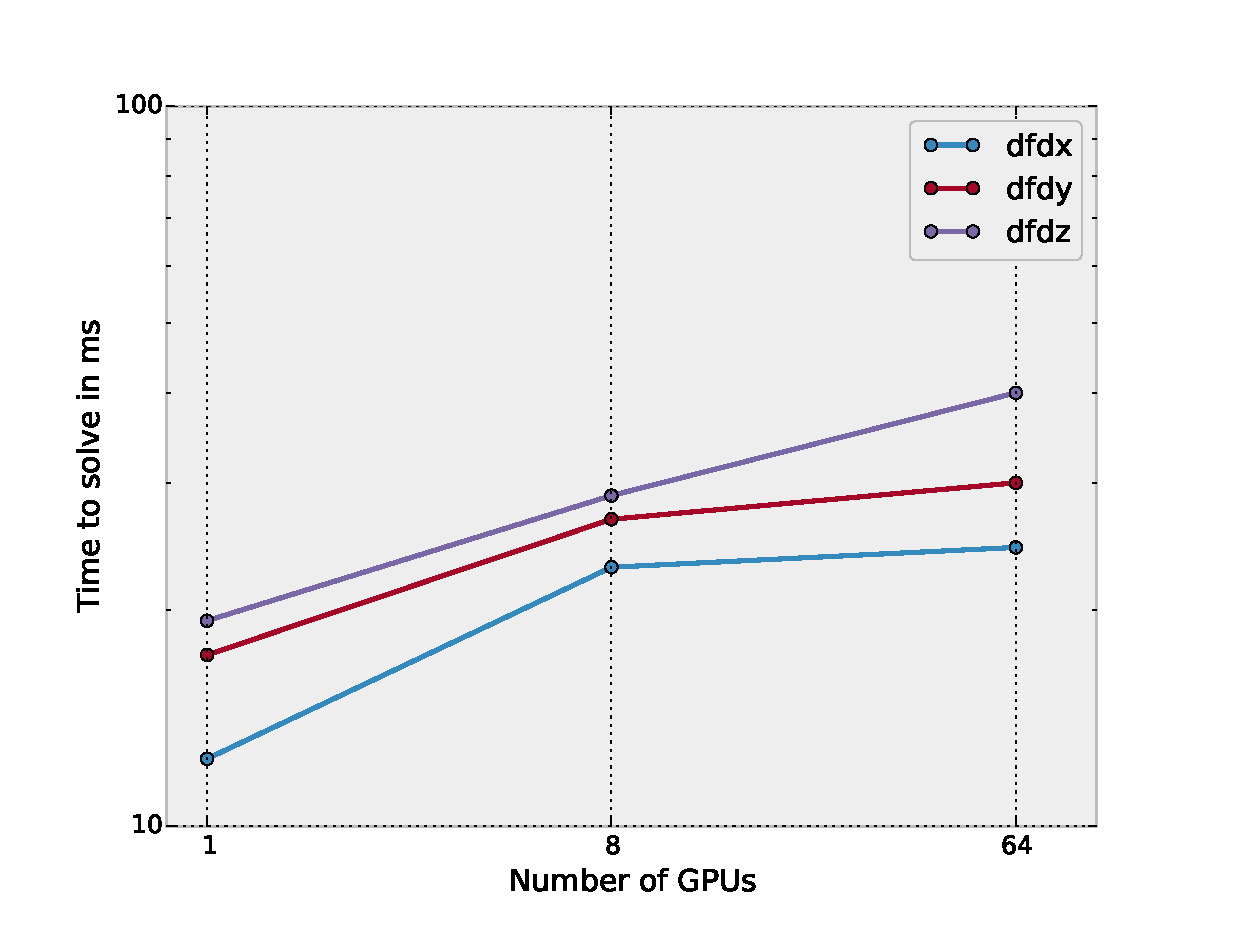
\includegraphics[width=300pt]{fig/weak-scaling-256.eps}
\caption{Weak scaling for multi-GPU compact finite difference, problem size: $256^3$ per process.}
\label{fig:weak-scaling-256}
\end{center}
\end{figure}
%
Figures \ref{fig:strong-scaling-256} - \ref{fig:weak-scaling-256}
show the strong and weak scaling of the compact finite difference solver
for evaluating derivatives in all three coordinate directions.
For the strong scaling measurement,
we keep the problem size fixed
and increase the number of GPUs used to solve the problem.
For the weak scaling measurement,
we keep the problem size \emph{per GPU}
fixed, and increase the number of GPUs used.
We note good scaling for both 2-D and 3-D cases.
The strong scaling for 3-D problems is somewhat better
as the GPU is kept busy for all problem sizes.

\subsection{Comparison with a CPU-only approach}

\centering
\begin{tabular}{|l|l|l|l|l|l|l|}
\hline
\multirow{2}{*}{Size} & \multicolumn{3}{c|}{Ref. impl, \#CPU cores} & \multicolumn{3}{c|}{NEATO-based, \#GPUs} \\ \cline{2-7}
         & 8         & 64        & 512      & 1       & 8       & 64      \\ \hline
$256^3$  & 79.5      & 20.8      & 11.1     & 19.9    & 5.17    & 2.79    \\ \hline
$512^3$  & 556.8     & 146.5     & 29.2     & 164.5   & 23.24   & 5.62    \\ \hline
$1024^3$ & 5188      & 1092      & 223.7    & -       & 174.9   & 24.49   \\ \hline
$2048^3$ & -         & -         & 1741     & -       & -       & 297.07  \\ \hline
\end{tabular}

%
\begin{figure}
\begin{center}
\includegraphics[width=300pt]{fig/compact-refimpl-speedups.eps}
\caption{Speedups over reference implementation
    for computing derivative in the fastest coordinate direction}
\label{fig:compact-refimpl-speedups}
\end{center}
\end{figure}

We also compare the performance of our compact finite difference
solver with the approach described by
Mohd-Yusof et al.\ \cite{mohd2010adapting},
implemented for CPUs.
The approach uses a distributed tridiagonal solver based on
the LU decomposition specialized for tridiagonal systems.
The problem is divided among individual CPU cores,
communicating via MPI.
For comparing timings,
we use the number of CPU sockets as the basis.
Each CPU socket uses 8 CPU cores and 1 GPU.
Thus, we maintain a ratio of 1:8 between GPUs and CPU cores
in our comparison.
Table \ref{table:compact-refimpl-timings}
shows timings for computing derivatives
in the fastest coordinate direction
for problems sized up to $2048^3$,
and Fig. \ref{fig:compact-refimpl-speedups}
shows the respective speedup using our implementation.


\end{document}

